
\chapter{\uppercase{Proposed Surrogate Training and Validation Framework}} 
\label{TPSFramework}

The previous two chapters discussed the drawbacks associated with prevalent DoE and error estimates for surrogate models.
In this chapter a unified framework for training point selection and error estimation for surrogate models is proposed. 
 The fundamental driver of the framework is the information available from local surrogate models built over sub-domains of the main surrogate model.
The local surrogate models refer to the ones that are built over the sub-domains of the global surrogate, using only a portion of the available data.
% The reason for constructing local approximations instead of multiple global approximations is to keep the computational cost low, as it is relatively cheap to build local surrogate models with only a few training points over a smaller domain at a fraction of computational cost.
A detailed account on the proposed dynamic training point selection and error estimation framework is provided in the following paragraphs.

%The global surrogate model refers to the main surrogate model that is built over the entire domain of interest whereas the local surrogate model refers to the ones that are built over sub-domains of the main surrogate. 
%Building auxiliary local surrogate models for sub-domains of the global surrogate model forms the basis of the framework. 
\section{Discussion of Steps Involved}
\label{dynamic}
Figure~\ref{flowchart} shows a schematic diagram of the algorithm.
\begin{figure}[h!]
\centering
\begin{minipage}[b]{0.95\linewidth}
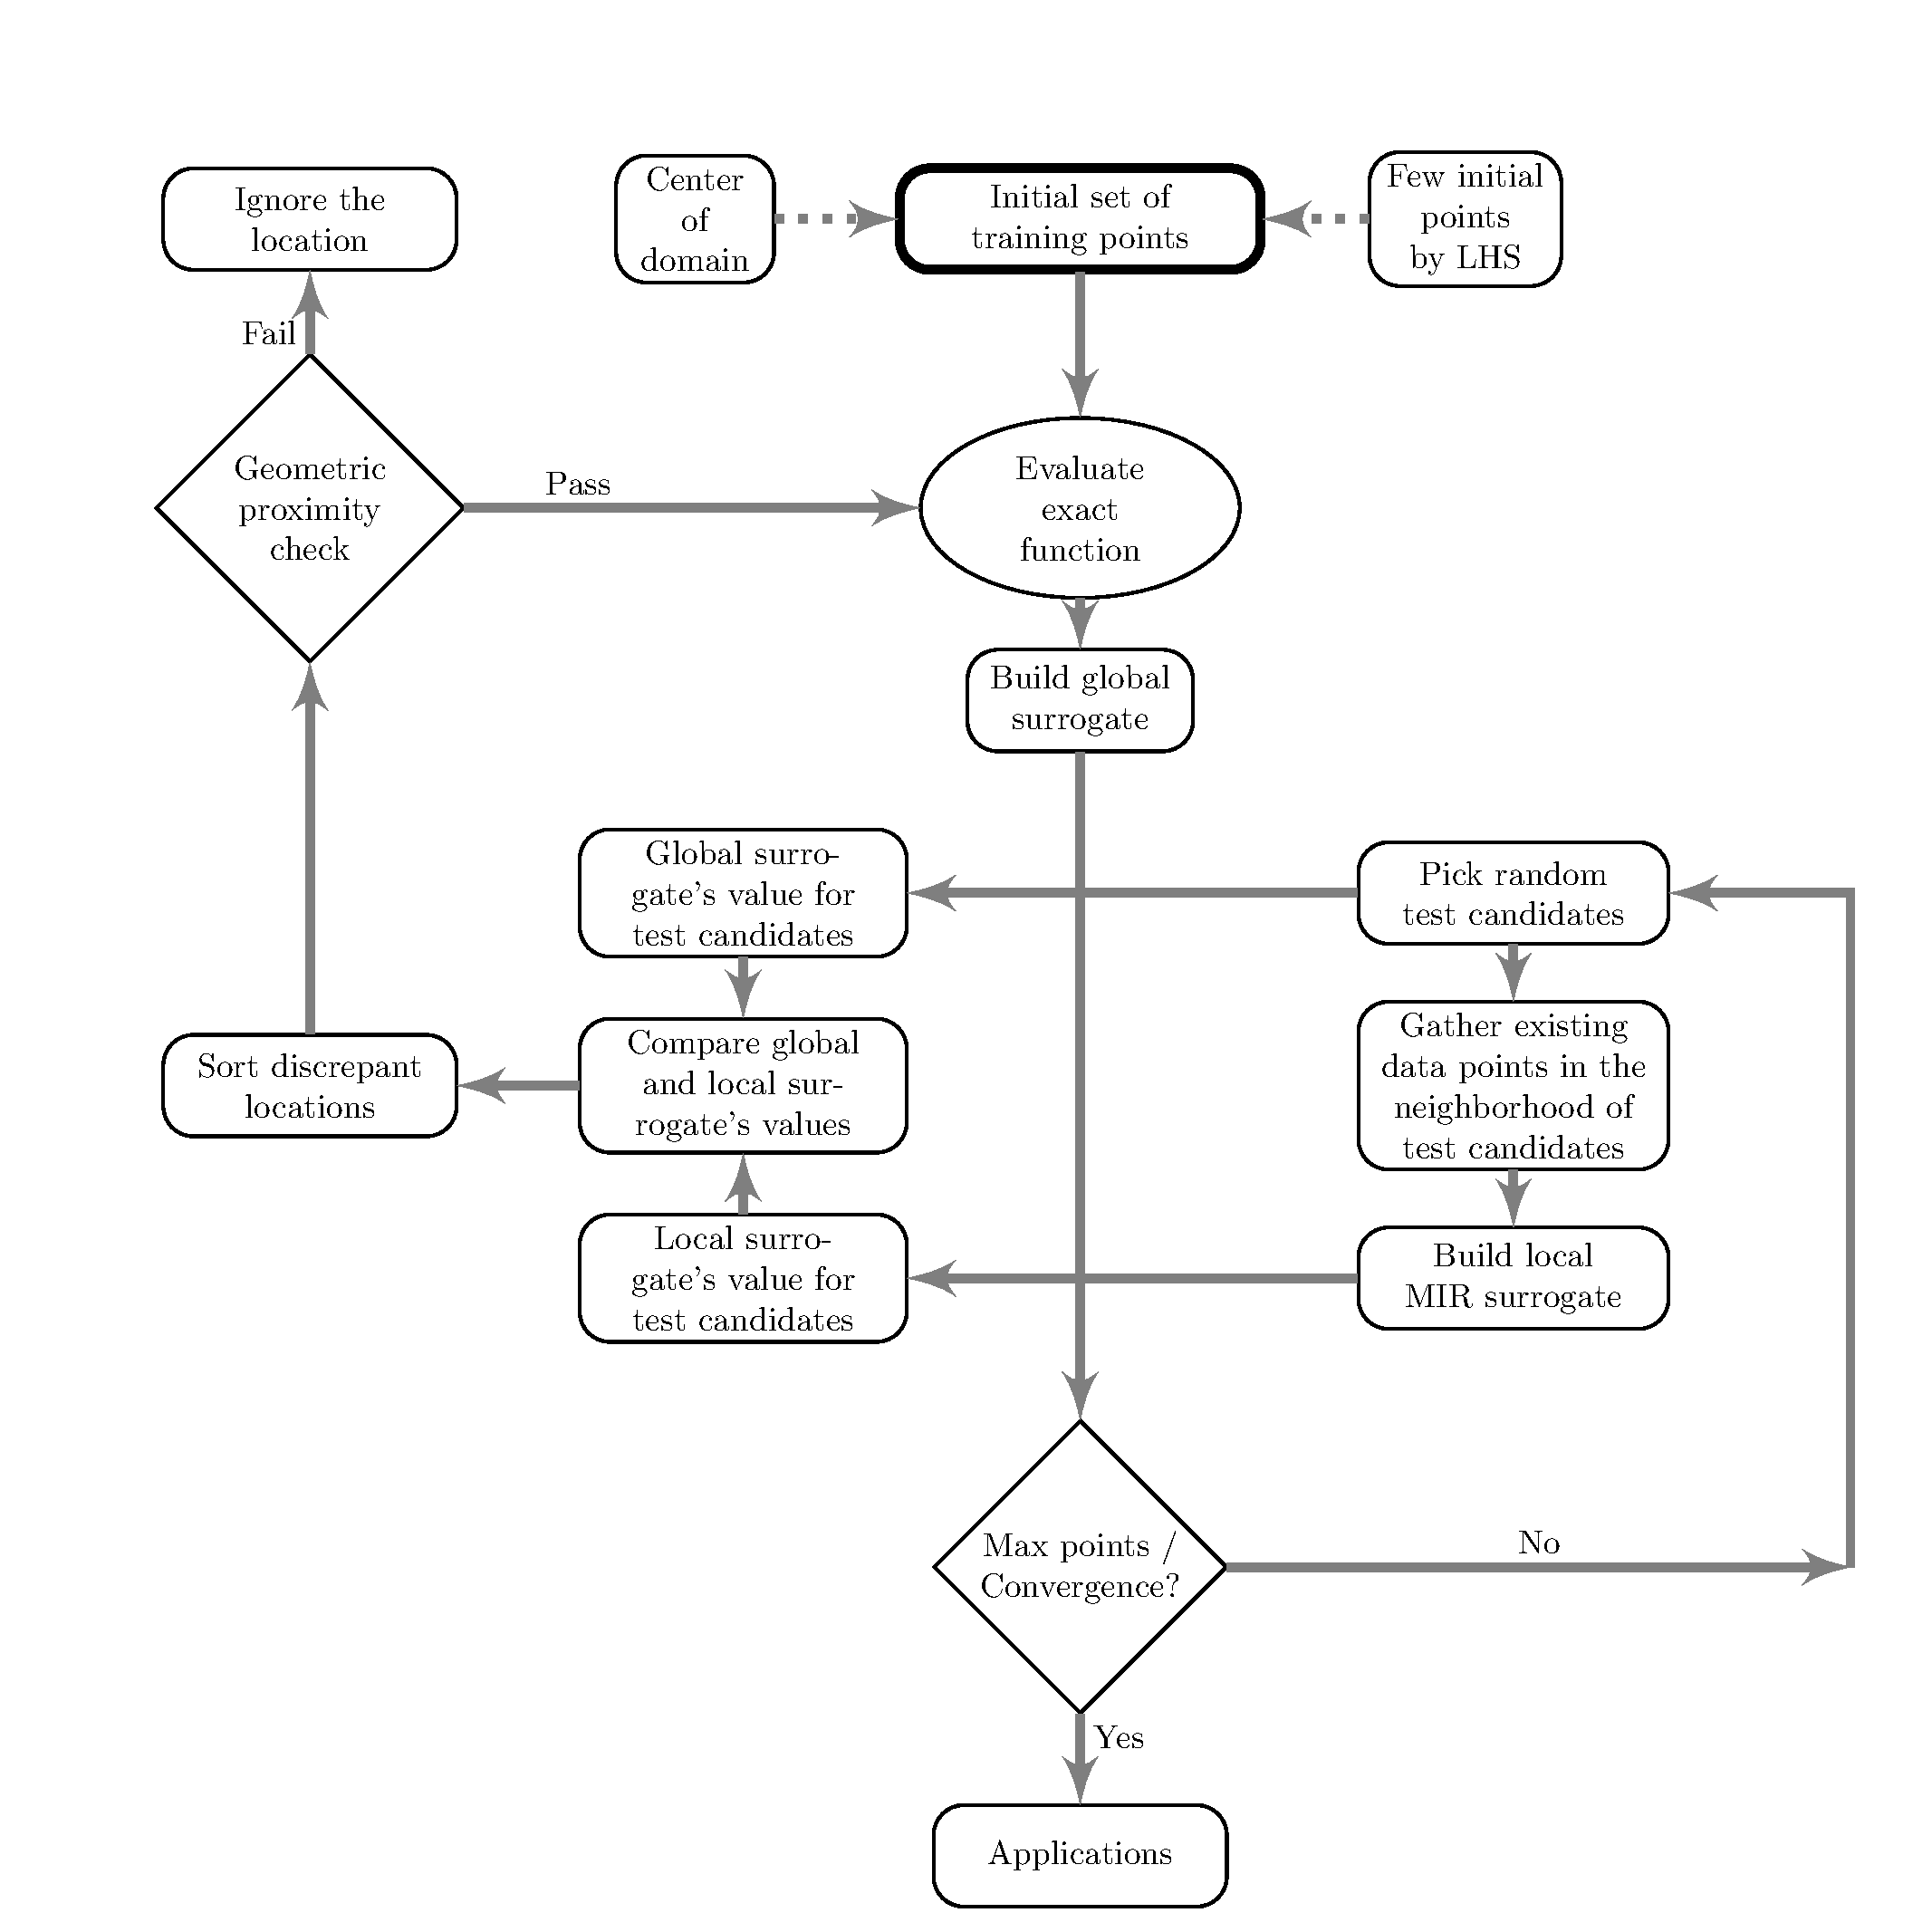
\includegraphics[width=1.0\textwidth,clip=true,trim=0.0in 0in 0in 0.70in]{flowchart.eps}
\end{minipage}
\caption[A schematic diagram of the proposed framework.]{A schematic diagram of the proposed framework for training point selection using a local surrogate (MIR).}
\label{flowchart}
\end{figure}
%Right  Bottom  Left Top --> If you want to trim the figure to fit your slides. Minor tweeks should be able to make it fit perfectly, if needed.
The steps involved in the process are as follows.

\subsection*{I.~Initialization}\label{initializing} 
The exact function (also gradient and Hessian, if desired) is evaluated at the center of the domain and a few other points picked by LHS, totaling \nom{$N_{init}$}{number of training points for the initial surrogate} training points.
The choice of $N_{init}$ is left to the user; however, it is recommended to start with a reasonably small number depending on the dimensionality and size of the domain.
In this work, for two-dimensional test cases, $N_{init}$ has been set to five for kriging and twelve for PCE, where the latter includes an oversampling factor of two and the required number of data points to build a second-order PCE
(setting $p=2$ and $M=2$ in Eq.~\ref{numberofterms}). For five-dimensional test cases, $N_{init}$ is set to fifty for kriging and forty-two for PCE.

\subsection*{II.~Evaluation of Surrogate Models}\label{evaluating}

Numerous test candidates, $\z^{(j)},\;j=1,\ldots,N_{test}$, are picked throughout the entire domain via LHS and the following is done with the two surrogates:

  \begin{enumerate}[(a)]
  \item \textbf{Global surrogate:}~The global surrogate model, which is built using all available training data, is simply evaluated at all these test candidate locations yielding $\widehat{f}_{global}^{(j)}(\z),\;j=1,\ldots,N_{test}$ and the values are stored. 

  \item \textbf{Local surrogate:}~During the first selection cycle, only one local surrogate is built using all available $N_{init}$ training data points (making it a ``second global surrogate''). 
The local surrogate model is also simply evaluated yielding $\widehat{f}_{local}^{(j)}(\z), \;j=1,\ldots,N_{test}$.
    During subsequent selection cycles, local surrogate models are rebuilt using $N_{local}$ closest existing training points for each test candidate $\z^{(j)}$ to evaluate $\widehat{f}_{local}^{(j)}(\z)$.
  \end{enumerate}
  In practical applications, it is intractable to evaluate the exact function to calculate the root mean square error of the global (main) surrogate model.
  A discrepancy function \nom{$\delta{(\z)}$}{discrepancy function at a test location} is proposed as an approximation to the actual error \nom{$\epsilon(\z)$}{actual error at a test location} between the exact function and surrogate model at any given location $\z$, and is defined as the absolute difference in predictions from global and local surrogate models:~$\delta(\z)=|\widehat{f}_{global}(\z)-\widehat{f}_{local}(\z)|$. 
  The underlying assumption is that the local surrogate models provide a more accurate representation of \emph{their corresponding sub-domain} than the global surrogate model since 
  piecewise approximations are generally considered to be more accurate for highly non-linear and non-smooth functions~\cite{Piecewise1,Desai2013}.
  Though the local surrogate models can be inaccurate in some cases, for example, due to scarcity of training data, extrapolations in unbounded space, improper tuning of the parameters for the local models, etc., 
  they can still serve as reference models for the global surrogate model.
In the same context of discussion, multiple local approximations can also be constructed with yet another local surrogate model (e.g. radial basis functions~\cite{Buhmann2005}, neural networks~\cite{NeuralNetworks}) 
  in addition to the MIR local surrogate for added fidelity, but this avenue is not explored in this work.

 \paragraph{Proposed error measures:} As discussed in chapter~\ref{validation}, actual surrogate model error estimates such as RMSE and MAE are prohibitively expensive to obtain.  A brief note on RMSE and MAE has been provided in section~\ref{sec:withrealevals}. In order to validate the surrogate models in applications of practical interest two error estimates are proposed:
\begin{enumerate}[(a)]
\item A \emph{root mean square discrepancy} (RMSD) defined as:
  \beq
  \textrm{RMSD}={\sqrt{\frac{1}{N_{test}}{\sum_{j=1}^{N_{test}}(\widehat{f}^{(j)}_{global}-\widehat{f}^{(j)}_{local})^2}}}={\sqrt{\frac{1}{N_{test}}{\sum_{j=1}^{N_{test}}(\delta^{(j)})^2}}},
  \label{eq:RMSD}
  \eeq
 can be used as an approximation to the actual root mean square error (RMSE or $L_2$-norm) of the surrogate model.

  %  \subsubsection*{Maximum Absolute Discrepancy}\label{sec:mad}
\item  Similarly, a \emph{maximum absolute discrepancy} (MAD) defined as:
  \beq
  \textrm{MAD}=\textbf{max}\{|\widehat{f}_{global}^{(j)}-\widehat{f}_{local}^{(j)}|\}\qquad j=1,\ldots,N_{test},
  \label{eq:MAD}
  \eeq
  measures the worst discrepancy between the local and global surrogate models and can be used to emulate the actual maximum absolute error (MAE or $L_\infty$-norm).
\end{enumerate}

\paragraph{Remark 1:}The data used for building the local surrogate models is a subset of already available data, $f^{(i)}(\x),~i=1,2\ldots,N$. Thus, no additional exact function evaluations are needed for constructing the local surrogates.
\paragraph{Remark 2:}Although the number of training points used to build a local surrogate, \nom{$N_{local}$}{number of training points for the local surrogate}, can be as high as the number of points used to build the global surrogate, $N$, it is recommended 
to only use a $N_{local}$ that is sufficient to produce a reasonably accurate local surrogate model. 
As a rule of thumb, studies similar to the ones shown in section~\ref{prelims} can be used to assess the accuracy of the local surrogate models. When it is not possible to determine the accuracy of the local surrogate models a priori (as in most scenarios), a certain percentage of the available training data (e.g. $25\%$) can be allocated for training the local surrogate models.  
In this work, 5--50 closest existing data points (depending on the dimension of the problem) are used to build the local surrogate models.
Using more points to increase the accuracy of the local surrogate model will also increase the computational expenses in building and evaluating it.
\paragraph{Remark 3:}The user should choose an appropriate number of test candidates, $N_{test}$, depending on the dimensionality of the surrogate. 
For example, heuristics used for Monte Carlo~\cite{Sobol94} or inexpensive Monte Carlo simulations~\cite{Yamazaki2012} (IMCS) can be adopted. 
In this work 1,000--25,000 test candidates are used. 
A larger \nom{$N_{test}$}{number of test candidates} facilitates a much wider exploration of the domain but comes with a higher cost. 
Fortunately, building and evaluating the local surrogates can be executed in parallel.
As each \textit{test candidate} is a \textit{potential training point location} during the next selection cycle, these terms will be used synonymously.

\subsection*{III.~Selection of Training Points}\label{selecting}

Selection is the process that determines whether or not a test candidate becomes a training point at which the exact function (gradient and Hessian) is to be evaluated. This includes the following two steps:

%\begin{enumerate}
\begin{enumerate}[(a)]
\item \textbf{Sorting the discrepancies:}
%\subsubsection*{(a)~Sorting the Discrepancies}
Locations (test candidates) are prioritized based on calculated discrepancies between the global and local surrogate model predictions.
A sorted discrepancy function vector contains values in the order of decreasing discrepancy and is represented as $\bm{\delta}_{sort}(\z)$. 
%\subsubsection*{(b)~Proximity Check}\label{proxcheck}
\item\label{proxcheck} \textbf{Proximity check:}
The distance, \nom{${\rho}^{(j)}$}{distance between $j$-th test candidate and its closest training point}, between each test candidate, $\z^{(j)}$, and its nearest existing training point, \nom{$\x^{*(j)}$}{closest training point to $j$-th test candidate}, is calculated. 
Mathematically,
\begin{equation}\label{eq:mindist}
\begin{aligned}
& {\rho}^{(j)}(\z^{(j)},\x^{*(j)})=||\z^{(j)}-\x^{*(j)}||_2, \;\; j=1,\ldots,N_{test}.& & \\
\end{aligned}
\end{equation}
%where $\bm{\rho}^{(j)}$ measures the distance between the $j-$th test candidate to its closest existing training point.
The mean value of all these distances measures the average proximity of a potential training point (belonging to the set of test candidates) to an existing training point and is written as,
\begin{equation}\label{eq:avgmindist}
\begin{aligned}
& \bar{\rho}=\frac{1}{N_{test}}\sum_{j=1}^{N_{test}}{\rho}^{(j)}.& &  \\
%& \forall \z \; \in \z^{(i)}, \; i=1,\ldots,N_{test},& & \\
\end{aligned}
\end{equation}
Now, each test candidate from the ordered set, $\bm{\delta}_{sort}(\z)$, starting with the one with the largest discrepancy is checked 
for proximity to already existing training points by calculating whether $\rho^{(j)}>c\bar{\rho}$, where \nom{$c$}{control parameter for distance-constraint} is a \emph{control parameter} that can be specified by the user to relax or strongly emphasize the constraint. 
 If a particular test candidate passes the check, it is added to the actual set of training points and the exact
function (gradient and Hessian) is evaluated.
After every successful selection of a training point the distances given by Eqns.~(\ref{eq:mindist}) and (\ref{eq:avgmindist}) are updated.
\end{enumerate}
The proximity check is repeated until \nom{$N_{cyc}$}{number of training points selected per cycle} new training points have been selected at this selection cycle. 
The newly available training data can now be used in subsequent selection cycles of the framework to update the surrogate models.
%, are obtained and the process is now returned to Step~(\ref{evaluating}).
%The first $N_{cyc}$ points to comply with Eq.~\ref{eq:selection} are added to the training point set and the exact function (gradient and Hessian) is evaluated.
\paragraph{Remark 4:}The enforcement of a geometric constraint works under the assumption that the global surrogate model is sufficiently accurate within $c\bar{\rho}$ distance from an existing training data point. 
In other words, the main surrogate does not warrant any additional training data within this radius, and the exact function can rather be evaluated at a more unexplored location. 
This criterion ensures that the training points are not clustered in one particular region and are sparse in other regions of the domain.
As already mentioned in chapter~\ref{introduction} each function evaluation can be computationally very expensive, especially for high-fidelity physics-based simulations, 
and it is essential to effectively choose each new training point.
\paragraph{Remark 5:} The availability of gradient and Hessian information affects the local as well as global surrogate model's approximation. It influences the discrepancy function $\delta$ driving the framework and helps the user in identifying the most viable locations to evaluate the derivative information.

\paragraph{Remark 6:}Due to the enforcement of the geometric constraint the framework may not support \textit{fast} optimizations as these constraints can prevent the placement of many training points close to the optimum. 
Though the framework is recommended for building globally accurate surrogate models, the geometric constraints do not severely restrict the applicability to optimizations as they are controllable by means of the control parameter $c$.

\subsection*{IV.~Termination}\label{terminating} 

Steps (II) and (III) are repeated to iteratively update the global and local surrogate models until any one of the following criteria is satisfied.

\begin{enumerate}[(a)]

\item{\textbf{Reach desired accuracy:}}\label{convcriterion} 
      The maximum absolute discrepancy (MAD) and/or root mean square discrepancy (RMSD) can be used to monitor the estimated accuracy of the current surrogate.
    A close agreement between MAD and MAE  as well as RMSD and RMSE will be shown in sections~\ref{rmsddemo} and~\ref{rmsddemoCFD}.
    The process of selecting additional training data can be stopped when the desired accuracy is reached.
  

\item{\textbf{Exhaust computational budget:}}
 % Usually a computational budget is  when applying surrogate models to applications of practical interest. 
When a maximum number of exact function (gradient and Hessian) evaluations is reached the user can stop the training point selection process.
  %
\end{enumerate}

\paragraph{Remark 7:} The framework can simply be used for surrogate model error estimation by skipping the third step (Selection of Training Points).




\section{Choice of Local Surrogate Model}\label{prelims}

This section provides guidelines on choosing a good local surrogate model that can guide the framework effectively. The following discussions are directed on establishing the suitability of multivariate interpolation and regression (MIR) in serving as local surrogate model.

\subsection{Ordinary Kriging and MIR}


Figure~\ref{KVM2D} compares the original kriging and MIR on two-dimensional exponential, Runge, and Rosenbrock test functions (see section~\ref{testcases} for their definitions), where all training points are selected through LHS.
%For this experiment, the Taylor order of MIR is set equal to the number of training points $(N)$ when only function values are used and it is set to $3{N}$ when both function and gradient information are used.
The general observation is that MIR approximates all test functions except Runge better than kriging.
The addition of gradient information for surrogate training (labeled FG, continuous lines) yields better results than training with function values alone (labeled $F$, dotted lines).
The reader is referred to Wang \etal~\cite{Qiqi2010a,Qiqi2010b} for a detailed comparison of MIR with other surrogate modeling methods and higher-dimensional test functions.

\begin{figure}[h]
  \centering
\begin{minipage}[b]{0.32\linewidth}
  \includegraphics[width=1.0\textwidth]{kvmexp.eps} \subcaption{Exponential}
\end{minipage}
\begin{minipage}[b]{0.32\linewidth}
  \includegraphics[width=1.0\textwidth]{kvmrun.eps} \subcaption{Runge}
\end{minipage}
\begin{minipage}[b]{0.32\linewidth}
  \includegraphics[width=1.0\textwidth]{kvmrosen.eps} \subcaption{Rosenbrock}
\end{minipage}
\caption[Comparison of kriging and MIR.]{Plots of RMSE of the surrogate versus the number of training points using kriging and MIR on two-dimensional test functions.}
\label{KVM2D}
\end{figure} 
\subsection{Effect of Taylor Order}
\begin{figure}[h]
\centering
\begin{minipage}[b]{0.32\linewidth}
   \includegraphics[width=1.0\textwidth]{exptaylor.eps}  \subcaption{Exponential}
\end{minipage}
\begin{minipage}[b]{0.32\linewidth}
  \includegraphics[width=1.0\textwidth]{runtaylor.eps} \subcaption{Runge}
\end{minipage}
\begin{minipage}[b]{0.32\linewidth}
  \includegraphics[width=1.0\textwidth]{rosentaylor.eps} \subcaption{Rosenbrock}
\end{minipage}
\caption[Effect of Taylor order on MIR approximation.]{Plots of MIR-RMSE versus the number of training points for different Taylor orders, $n$, on two-dimensional test functions.}
\label{Taylor}
\end{figure}

Figure~\ref{Taylor} shows the effect of different Taylor orders on the
accuracy of the MIR approximated function value, $\widehat{f}$. 
It can be seen that a lower Taylor order, $n$, such as one or two produces a less accurate approximation, whereas a higher $n$ leads to an improved approximation. For the Rosenbrock test function, after a certain number of points, the MIR expansion accurately  models the function (close to machine precision).
The problem with a higher Taylor order is that it increases the computational time in building the MIR surrogate significantly and there is not an easy way to choose the appropriate Taylor
order a priori. It is recommended to use a Taylor order that is equal to the number of data points $(\ie~n=N)$ when only function values are used for model training, or $3N$ if the data points also contain gradient information~\cite{Qiqi2010a,Qiqi2010b}.

%\subsection{}

Building the MIR surrogate becomes computationally very expensive with  increasing number of training points.  It can be seen from Figure~\ref{KVM2D} that MIR is able to produce comparatively good surrogates with just a few training points and hence are cheaper to build.
%\paragraph{Kriging:}
It is generally acknowledged that, kriging has the capability to represent multi-modal functions and can effectively capture non-smooth functions~\cite{Yamazaki2010}. Moreover, kriging supports the usage of both high- and low-fidelity training points \ie~ a variable-fidelity kriging surrogate~\cite{Han2012,Han2012b,Han2009,Han2010,Yamazaki2013,Yamazaki2012,Yamazaki2011b} can be constructed. 
%\paragraph{Proposed usage of MIR:}
Due to these reasons kriging is preferred as the global surrogate model, whereas MIR is used to guide the training point selection process as well as to provide a metric for the accuracy of the global surrogate,  using the framework discussed in section~\ref{dynamic}.
